\subsection{Evaluation}\label{sec:evaluation}

Subsequent sub-chapters discuss metrics for evaluation and measures to retrieve feature importance estimates from the estimators.

\subsubsection{Evaluation Metric}\label{sec:evaluation-metric}

Our goal is to maximise the number of trades, where the predicted trade initiator matches the true trade initiator. We assess the quality of our model’s prediction in terms of \emph{accuracy}, which can be stated as:
\begin{equation}
    % \operatorname{accuracy} \colon \mathbb{R}^{N} \times \mathbb{R}^{N} \to  \left[0, 1\right], \quad 
    \operatorname{accuracy}(\mathbf{y}, \widehat{\mathbf{y}}) = 1 - \frac{1}{N}\sum_{i=1}^{N} \operatorname{L}_{\mathrm{0-1}}(\mathbf{y}_i, \widehat{\mathbf{y}}_i),
\end{equation}
where $\operatorname{L}_{\mathrm{0-1}}(\cdot)$ is the 0-1-loss given by:
\begin{equation}
    % \operatorname{L}_{0-1} \colon \mathcal{Y} \times \mathcal{Y} \to \left[0, 1\right], \quad 
    \operatorname{L}_{\mathrm{0-1}}(y, \hat{y}) = \mathbb{I}\left(y\neq \hat{y}\right).
\end{equation}

Intuitively, from the 0-1-loss we obtain the error rate on the dataset, as for every misclassified trade we count a loss of one and normalise by the number of samples $N$, which gives the normalised 0-1-loss. Notably, the loss is the same for false positives and negatives.

Our datasets are approximately balanced and buyer-initiated trades predicted as seller-initiated and vice versa have similar associated costs, which makes accuracy an ideal choice as a performance metric.\footnote{The \gls{ISE} test set consists of \SI{48.5973}{\percent} of buy trades and \SI{46.1278}{\percent} of the \gls{CBOE} test set are buy trades.} As the 0-1-loss and in consequence, the accuracy is not differentiable, it cannot be used in optimisation, but as an early stopping criterion to halt training or as an optimisation target in the hyperparameter search. We report the accuracy of the test sets.

\subsubsection{Feature Importance
    Measure}\label{sec:feature-importance-measure}

Naturally, we aim to gain insights into the prediction process and identify relevant features, which fall under the umbrella of \emph{interpretability}.
Following, \textcite[][4]{liptonMythosModelInterpretability2017} interpretability can be reached through model transparency or post-hoc interpretability methods. Transparent models provide interpretability through a transparent mechanism in the model, whereas post-hoc methods extract information from the already learnt model \autocite[][4--5]{liptonMythosModelInterpretability2017}.

Classical trade classification algorithms, as a rule-based classifier, are transparent with an easily understandable decision process and thus provide interpretability \autocite[][91]{barredoarrietaExplainableArtificialIntelligence2020}. Interpretability, however, decreases for deep, stacked combinations involving a large feature count, when interactions between base rules become more complex and the effect of a single feature on the final prediction more challenging to interpret.

The machine-learning classifiers, studied in this work, can be deemed a black box model \autocite[][90]{barredoarrietaExplainableArtificialIntelligence2020}. Due to the sheer size of the network or ensemble, interpretability through transparency is impacted. Albeit, the attention mechanism of Transformers provides some interpretability through the attention mechanism,  interpretability across all classifiers can only be reached through \emph{model-agnostic, post-hoc interpretability techniques}.

Thereby, our goal is to estimate how much a feature contributes to the performance of the classifier \emph{overall}, which urges for \emph{global feature attribution measures}. The appropriate approach is guided by the properties of the data. Due to the data-generating process with strongly correlated quotes and trade prices at the exchange and nationwide levels, features are strongly dependent. The redundant feature encoding of ratio features exacerbates this effect. Feature independence, however, is the central assumption of most popular feature importance measures, including \gls{SHAP}, \gls{LIME}, or random feature permutation \autocite[][2]{aasExplainingIndividualPredictions2021}. A violation of this constraint for two perfectly correlated, predictive features can have the effect that both are deemed unimportant as the feature importance is distributed between features underestimating the true importance of the feature \autocite[][4]{covertUnderstandingGlobalFeature2020}.

For this reason, we estimate feature importances using \gls{SAGE}, which can account for complex interactions between features and yields global importances. 

\textbf{Shapley Additive Global Importance}


\textbf{Attention Maps}

In addition to permutation-based methods, Transformer-based models offer \emph{some} interpretability through their attention mechanism. In recent research a major controversy embarked around the question, of whether attention offers explanations to model predictions \autocites[cp.][150]{bastingsElephantInterpretabilityRoom2020}[][5--7]{jainAttentionNotExplanation2019}[][9]{wiegreffeAttentionNotNot2019}. The debate sparked around opposing definitions of explainability and the consistency of attention scores with other, established feature-importance measures. Our focus is less on post-hoc explainability of the model, but rather on transparency. Consistent with \textcite[][8]{wiegreffeAttentionNotNot2019} we view attention scores as a vehicle to model transparency.

Recall from our discussion on attention (cp. \cref{sec:attention}) that the attention matrix stores how much attention a token pays to each of the keys. Thus, feature attributions can be derived from attention by visualising features to which the model attends to in an attention map. While attention maps are specific to Transformers or other attention-based architectures, rendering them useless for cross-model comparisons, they give additional insights from different attention layers and attention heads of the model on a per-trade and global basis. % An example is shown in \cref{fig:attention-maps}.

% \begin{figure}[ht]
%     \centering
%     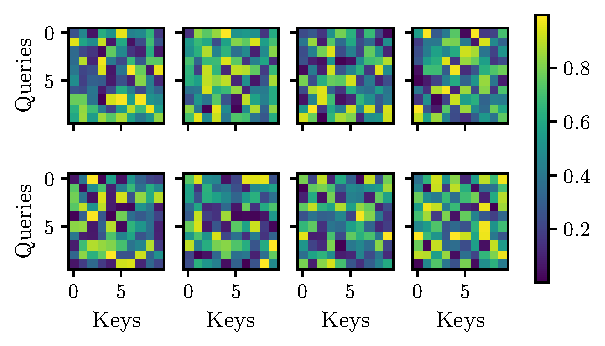
\includegraphics{attention-maps.pdf}
%     \caption[Attention Maps]{Attention Maps.}
%     \label{fig:attention-maps}
% \end{figure}

In the tabular domain, various approaches have been investigated in the literature to obtain attention from multiple attention heads and Transformer blocks. \textcite[][18]{somepalliSaintImprovedNeural2021} and \textcite[][11]{borisovDeepNeuralNetworks2022} gather attention maps from the first attention layer only, and \textcite[][11]{borisovDeepNeuralNetworks2022} additionally obtain feature attributions by taking the diagonal of the attention matrix $\mathbf{A}$ or through column-wise summation. In contrast, \textcite[][10]{gorishniyRevisitingDeepLearning2021} leverage all attention matrices by averaging over multiple Transformer blocks, attention heads, and samples to obtain global feature attributions. Given \cref{sec:architectural-overview,sec:attention}, where we emphasised the unique role of attention heads and lower sub-layers, both approaches may be myopic, as attention heads may contribute unequally to the result, or as later attention layers are neglected altogether.

While not explored systematically in the tabular domain yet, the rollout attention method of \textcite[][3]{abnarQuantifyingAttentionFlow2020} combines raw attention from multiple layers through recursive matrix multiplication with the weight matrices from attention layers below, as shown in this Equation:\footnote{Notation from adapted from \textcite[][786]{cheferTransformerInterpretabilityAttention2021}.}
\begin{equation}
    \begin{aligned}
        \hat{\mathbf{A}}^{(l)}    & =\mathbf{I}+\mathbb{E}_h \mathbf{A}^{(l)}                                              \\
        \operatorname { rollout } & =\hat{\mathbf{A}}^{(1)} \cdot \hat{\mathbf{A}}^{(2)} \ldots\cdot\hat{\mathbf{A}}^{(L)}
    \end{aligned}
    \label{eq:attention-map-rollout}
\end{equation}

In each layer the raw attention scores $\mathbf{A}^{(l)}$ are averaged over $h$ heads, denoted by $\mathbb{E}_h$. The identity matrix $\mathbf{I}$ is added to account for the residual connections (\cref{sec:residual-connections-layer-norm}). While rollout attention considers all attention layers in the calculation of feature attributions, it does not consider a signal and attributes equal weights to all attention heads \autocite[][786]{cheferTransformerInterpretabilityAttention2021}.

In an attempt to explain the decision-making process of multi-modal Transformers, including self-attention-based Transformers, \textcite[][3]{cheferTransformerInterpretabilityAttention2021} incorporate gradients to weight the head's contribution when averaging over the heads of a layer, as shown in \cref{eq:attention-map-weighted}. Like before, all attention layers are considered.

\begin{equation}
    \begin{aligned}
        \bar{\mathbf{A}}^{(l)}   & =\mathbf{I} + \mathbb{E}_h\left(\left(\nabla \mathbf{A}^{(l)} \odot \mathbf{A}^{(l)}\right)^{+}\right) \\
        \operatorname {wrollout} & =\bar{\mathbf{A}}^{(1)} \cdot \bar{\mathbf{A}}^{(2)} \ldots \cdot \bar{\mathbf{A}}^{(L)}
    \end{aligned}
    \label{eq:attention-map-weighted}
\end{equation}

In this approach, the element-wise product between the gradient of the attention map $\nabla \mathbf{A}^{(l)}=\frac{\partial y_t}{\partial \mathbf{A}}$ for the model's target class $t$ and the attention map $\mathbf{A}^{(l)}$ is calculated to weight the attention head's importance. As previously suggested in \textcite[][786]{cheferTransformerInterpretabilityAttention2021}, negative contributions are eliminated to focus on the positive relevance, and the results are averaged over the heads dimension. Like all other presented approaches \cref{eq:attention-map-rollout,eq:attention-map-weighted} can be computed with a single forward pass and is therefore computationally efficient.

In the absence of ground truth for the true feature attribution, we resort to attention maps using \cref{eq:attention-map-weighted}. The level of agreement between attributions from attention maps and \gls{SAGE} values by calculating Spearman's rank correlation between them.
